\chapter{Design and Methodology}

\section{Introduction}

In this chapter the design and methodology choices involved in this project will be presented. This project consists of five key stages (Figure ~\ref{fig:pipeline}). Each of these will be discussed in detail in this chapter. The five stages are:
\begin{itemize}
    \item \textbf{Data Collection and Filtering}\newline
    This stage involved collecting the Twitter data. The data was then filtered so it only contained tweets about hotels posted from Dublin.
    \item \textbf{Dataset Annotation}\newline
    This stage involved annotating the filtered dataset of tweets about hotels in Dublin.
    \item \textbf{Classification}\newline 
    In this stage of the project multiple supervised machine learning classifiers were trained with different feature representations.
    \item \textbf{Sentiment Analysis}\newline 
    This part of the project involved analysing the sentiment of those tweets that were classified as reviews.
    \item \textbf{Application within a Recommender System}\newline
    In this stage the sentiment scores produced were used to re-rank the results of the CoRE \cite{core2019} Recommender System.
\end{itemize}

\begin{figure}[h!]
\centering
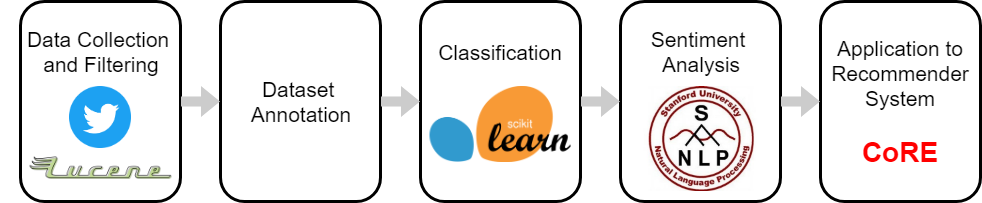
\includegraphics[width=1\textwidth]{design_and_methodology/pipeline.png}
\caption{\label{fig:pipeline} An overview of the key stages of the project.}
\end{figure}

\section{Data Collection}
The data was collected using the Twitter Streaming API \footnote{\url{https://developer.twitter.com}} (Application Programming Interface) between October 2017 and September 2018. Twitter has a Search API and a Streaming API. The Search API allows you to find historical tweets and the Streaming API allows you to stream real-time tweets.

The tweets used in this project were collected using the Streaming API. A location filter was specified so that only tweets posted from within the bounding box of Dublin were returned (Figure ~\ref{fig:dublinBB}). A total of 2.5 million tweets were collected.

After inspecting the collection of tweets it was found that although a bounding box had been specified, not all tweets in the collection had been posted from Dublin. A significant amount of tweets had slipped through Twitter's location filter. This meant that the first step required was to filter the dataset to ensure, as much as was possible, that all tweets related to Dublin.

\begin{figure}[h!]
\centering
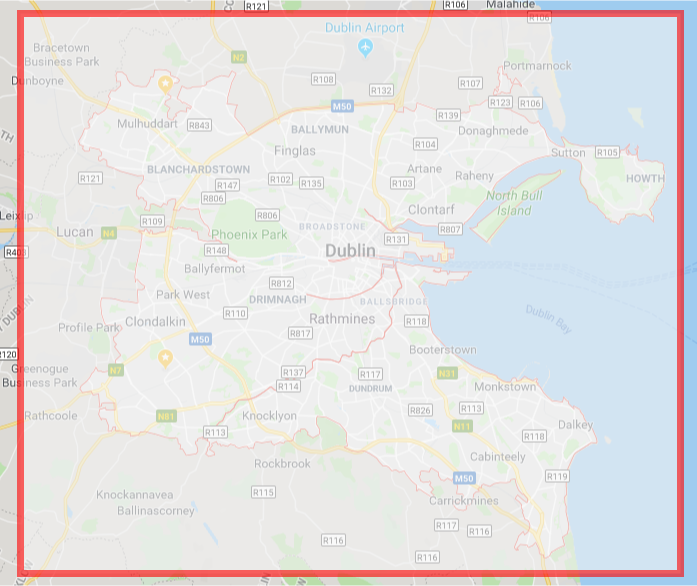
\includegraphics[width=0.75\textwidth]{design_and_methodology/dublinBB.png}
\caption{\label{fig:dublinBB} Bounding Box of Dublin.}
\end{figure}

\section{Data Filtering}

\subsection{Geo-tagged Tweets}

All of the tweets in the dataset were Geo-tagged because they were collected with a location filter. This meant they all had location data: a specified location from which the tweet was posted. There are two types of Geo-tagged tweets:
\begin{itemize}
    \item \textbf{Point Coordinate}\newline
    Tweets with a specific latitude/longitude or point coordinate. These tweets come from GPS enabled devices (Listing ~\ref{lst:pointjson}).
    \item \textbf{Twitter Place}\newline
    Tweets with a specified bounding box and Twitter Place. A bounding box is a four-sided geographic area, defined by four points of the form [longitude, latitude] (Figure ~\ref{fig:dublinBB}). This defines the general area the tweet was posted from (Listing ~\ref{lst:placejson}). \newline
\end{itemize}

\begin{lstlisting}[caption={Geo-tagged Tweet with Point Coordinate},
captionpos=b,label=lst:pointjson,language=json,firstnumber=1]
"geo": {
    "type": "Point",
    "coordinates": 
        53.28581863,
        -6.11439315
    ]
}
\end{lstlisting}

\begin{lstlisting}[caption={Geo-tagged Tweet with Twitter Place},captionpos=b,label=lst:placejson,language=json,firstnumber=1]
"place": {
  "full_name": "Dun Laoghaire-Rathdown, Ireland",
  "url": "https://api.twitter.com/1.1/geo/id/723427e351a01e72.json",
  "country": "Ireland",
  "place_type": "city",
  "bounding_box": {
    "type": "Polygon",
    "coordinates": [
      [
        [
          -6.282038,
          53.199283
        ],
        [
          -6.282038,
          53.315283
        ],
        [
          -6.066759,
          53.315283
        ],
        [
          -6.066759,
          53.199283
        ]
      ]
    ]
  },
  "country_code": "IE",
  "attributes": {},
  "id": "723427e351a01e72",
  "name": "Dun Laoghaire-Rathdown"
}
\end{lstlisting}

\subsection{Filtering Out Non-Dublin Tweets}

The first attempt to filter out any non-Dublin tweets used the point coordinates of the tweets. The point coordinate of each tweet was compared to the bounding box of Dublin. If it lay inside the box it was kept, otherwise it was filtered out. However, only 7.23\% of the tweets in our collection actually had a specific point coordinate. Filtering based on this excluded the majority of the dataset. To address this we instead filtered tweets based on a combination of their point coordinates and their Twitter places.

All of the tweets in the collection have a Twitter place defining the general area that the tweet was posted from. A combination of the Twitter place and the point coordinates was used to filter out any non-Dublin tweets that had ended up in the dataset. 

\begin{table}[h!]
\caption{The coordinates of Dublin's Bounding Box.}
\label{tab:dublinbb}
\setlength\extrarowheight{5pt}
\begin{tabular}{|c|c|}
\hline
North Latitude  & 53.425210 \\ \hline
South Latitude  & 53.223430 \\ \hline
East Longitude & -6.043924 \\ \hline
West Longitude & -6.447485 \\ \hline
\end{tabular}
\end{table}

A bounding box for the Dublin area was defined (Table ~\ref{tab:dublinbb}). Tweets with a point coordinate and tweets with only a Twitter place were filtered differently:
\begin{itemize}
    \item \textbf{Point Coordinate}\newline
    Each tweet with a point coordinate was checked to see if the point coordinate fell within the defined bounding box for Dublin. If it lay inside the box it was kept, otherwise it was filtered out.
    \item \textbf{Twitter Place}\newline
    Each tweet with a Twitter place has a bounding box specifying the location of the place. The centroid of this bounding box was calculated for each tweet. Then the centroid was checked to see if it fell within the defined bounding box for Dublin. If it lay inside the box it was kept, otherwise it was filtered out.
\end{itemize}

The filtered dataset consisted of 1.6 million tweets posted from Dublin between October 2017 and September 2018.

\subsection{Filtering Tweets About Hotels}

The dataset of tweets posted from Dublin now had to be further filtered. The next step was to extract all tweets that mentioned hotels.

A list of the hotels in Dublin was compiled. This included the hotel's name and the hotel's Twitter handles (@hotelname). This list consisted of 159 hotels and Twitter handles (Table ~\ref{Table:hotels}).

The tweets were stored in a Lucene index. A fuzzy search query was used to match the tweets against each of the hotel names and hotel Twitter handles. The fuzzy search query uses a similarity measure that is based on the Damerau-Levenshtein algorithm. The maximum edits option was set to two, meaning that strings with a maximum difference of two characters would still match. This accounted for misspellings and broadened our search slightly. We experimented with higher numbers of maximum edits but found that too many irrelevant tweets were returned.

No NLP (natural language processing) technique that attempts to identify all mentions will be 100\% accurate. Users will refer to hotels in all manner of ways, anaphora like 'the hotel'. We have tried to be reasonably conservative and ensure we have a pretty clean dataset, but there are a range of ways to identify hotels that could be experimented with. 
This further filtered dataset consisted of 3115 tweets that mention hotels posted from Dublin between October 2017 and September 2018. The distribution of tweets collected per hotel can be seen in the appendix (Table ~\ref{Table:tweetsperhotels}).

\section{Dataset Annotation}

One major goal of this research was to categorise tweets as review-like tweets, as tweets that contain some content and as irrelevant tweets. In order to train a classifier to do this a set of tweets had to first be manually annotated. The set of 3115 tweets about hotels in Dublin was annotated. This involved building an annotation webpage where users could view tweets and assign them labels.

\subsection{Annotation Webpage}

A simple webpage was created in order to annotate the tweets (Figure ~\ref{fig:webpage}). The webpage can be found at:
\begin{center}
    \url{http://reviewtweets.epizy.com}\newline
\end{center}

\begin{figure}[h!]
\centering
\fbox{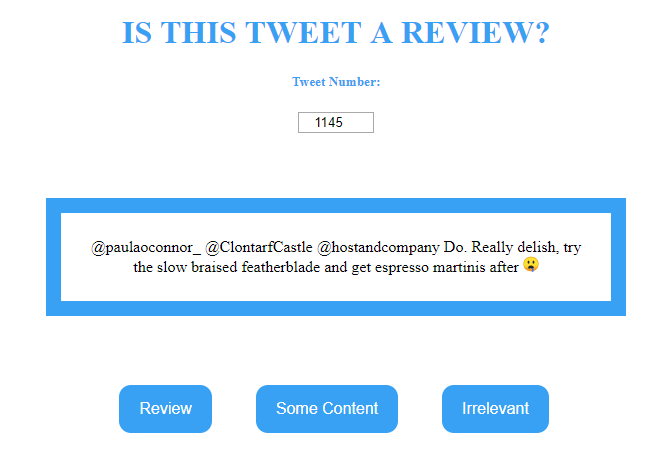
\includegraphics[width=1\textwidth]{design_and_methodology/webpage.PNG}}
\caption{\label{fig:webpage} Tweet Annotation Webpage.}
\end{figure}

The text of each tweet was displayed alongside three buttons: 'Review', 'Some Content' and 'Irrelevant'. The participant could click on the option that they thought best described the tweet shown. Once they chose a label, the next tweet would be displayed. 

Each time the webpage is loaded a random tweet from the dataset is displayed. This means each participant will label a different section of the tweets, ensuring all tweets in the collection get annotated evenly.

The following instructions, describing what a 'Review', 'Some Content' and 'Irrelevant' tweet should look like accompanied the webpage:
\begin{itemize}
    \item \textbf{Review} \newline
    The tweet could be considered as a review (of any aspects related to a hotel such as the venue, food, view, swimming pool, etc.) for any hotel. Examples would include: \emph{"Amazing view of the Aviva Stadium from my hotel balcony at hotel X"} (positive review), "Room service was awful at hotel Y" (negative review), \emph{"Thank you hotel X for a lovely stay"} (positive review) or \emph{"Had an awful night at hotel Y"} (negative review).
    \item \textbf{Some Content} \newline
    The tweet doesn't look like a review, but it does provide some information related to a hotel, such as the hotel hosts events, information on the menu, information related to accommodation, etc. Examples would include: \emph{"Hotel Z serves Tuna salad on Wednesday”} or \emph{“A packed room for the 2018 fashion conference at Hotel X”}.
    \item \textbf{Irrelevant} \newline
    This tweet is completely irrelevant. While perhaps mentioning the name of a hotel, the tweet doesn't give any additional information about that hotel or offer any opinions related to the hotel.
\end{itemize}

In this research we decided to focus solely on the text of the tweets. For this reason all images, videos and URLs were stripped from the tweets before being displayed on the annotation webpage. Images, videos and URLs could all carry valuable information and could be considered in future research. Image and video processing techniques could be experimented with to gather additional information from the tweets.   

\begin{table}[h!]
\caption{A sample of the tweets from the SQL table.}
\label{Table:TweetAnnotation}
\setlength\extrarowheight{5pt}
\resizebox{\textwidth}{!}{
\begin{tabular}{llllll}
\specialrule{1.5pt}{1pt}{1pt}
    \multicolumn{1}{l}{\textbf{Row No.}} & 
    \multicolumn{1}{l}{\textbf{Tweet ID}} & 
    \multicolumn{1}{l}{\textbf{Tweet}} & 
    \multicolumn{1}{l}{\textbf{Review}} & 
    \multicolumn{1}{l}{\textbf{Content}} & 
    \multicolumn{1}{l}{\textbf{Irrelevant}} \\ 
\specialrule{1.5pt}{1pt}{1pt}
\rowcolor[HTML]{EFEFEF} 
    1 & 00000 & 
    \begin{tabular}[c]{@{}l@{}}
        Creating A Rewarding Experience\\ 
        or CARE, essence of any\\ DoubleTree by Hilton hotels, \\ 
        is in the heart of everything in the\\ 
        Morrison Hotel! \#CARE \\
        \#DoubleTree \#dublincity \\ 
        \#brandculture
    \end{tabular} & 0 & 1 & 0 \\ 
\hline
    2 & 00000 & 
    \begin{tabular}[c]{@{}l@{}}
        @bfitzsimons @doubletree \\
        @DTHydePark Oohh. \\
        Impressed!
    \end{tabular} & 2 & 0 & 0 \\ 
\hline
\rowcolor[HTML]{EFEFEF} 
    3 & 00000 & 
    \begin{tabular}[c]{@{}l@{}}
        SlowMo Training \\ 
        \#EliteFest2018 @ The \\ 
        Morrison, a DoubleTree \\ 
        by Hilton Hotel
    \end{tabular} & 0 & 1 & 0 \\ 
\hline
    4 & 00000 & 
    \begin{tabular}[c]{@{}l@{}}
        Drinking a Heineken by \\ 
        @heineken at @doubletree —
    \end{tabular} & 0 & 2 & 0 \\ 
\hline
\end{tabular}}
\end{table}

The tweets were stored in a SQL table (Table ~\ref{Table:TweetAnnotation}) linked to the webpage, along with a count of the number of times the tweet had been labelled as a review, some content or irrelevant. Each time a participant chooses a label the corresponding value in the database is incremented. The final label of a tweet is determined by calculating which label had the maximum number of votes. 

The annotation webpage was circulated to friends, family and members of the Adapt Research Centre to gather annotations.

\section{Tweet Classification}

The annotated set of tweets was used to train a series of different classifiers to determine which classifier was most suited to the task. These classifiers were implemented using Python's Scikit Learn library \cite{scikit-learn}. The data was split into a training set and a testing set. The data was split 80:20 where 80\% was used for training and 20\% was used for testing.

\subsection{Data Pre-processing}

The set of annotated tweets was pre-processed before it was used to train the classifiers. The pre-processing stage tokenizes the tweets and deals with things like punctuation and case. The data pre-processing techniques used were inspired by the techniques found in previous literature \cite{Ankit2018,Rane2018,Go2009,Raithi2018}. 

The following steps were taken to pre-process the tweets, before they were used to train the classifiers:\newline
\begin{itemize}
    \item \textbf{Emojis}\newline
    Emojis were removed and replaced with text using Python's Emoji library \cite{emoji}. For example, a thumbs up emoji would be converted to the text \emph{':thumbs\_up:'} and then \emph{'thumbs up'} once punctuation is removed. In this way some meaning was extracted from each emoji. Emojis are another area of potential valuable sentiment information for future work. A. Go, R. Bhayani and L. Huang \cite{Go2009} used emojis to automatically label a dataset of tweets as positive or negative.
    \item \textbf{Punctuation}\newline
    The majority of special characters and punctuation was removed from the tweets. This included everything except the digits 0 - 9, the letters a - z (in upper and lower case), and the following set of symbols: . , ? ! ( ) \& ' - . Tweets are generally quite noisy and contain a lot of unnecessary punctuation. Symbols such as @ and \# were removed so that the words contained in hashtags and Twitter handles could be recognised as words. However, symbols like apostrophes were not removed so that a word like 'won't' wouldn't be split into 'won' and 't'.
    \item \textbf{Single Characters}\newline
    All single characters were removed. The majority of the single characters in the tweets were typos or added no extra meaning to the text. The only single character words are 'I' and 'a'. These are both stop words which are later removed anyway.
    \item \textbf{Case Change}\newline
    Words were split on case changes. For example \emph{'MerrionHotel'} --> \emph{'Merrion Hotel'}. This was because we noticed a lot of Twitter handles and hashtags contain words joined together without space. 
    \item \textbf{Word-digit Boundaries}\newline
    Words were split on word-digit boundaries. For example \emph{'HouseDublin2'} --> \emph{'House Dublin 2'}. Again, a lot of Twitter handles and hashtags contain words and digits joined together without space. 
    \item \textbf{Lowercase}\newline
    All text was converted to lower case. This is so that a word with a capital letter and a word without a capital letter are recognised as the same word.
    \item \textbf{Stemming}\newline
    Stemming was performed using the Word Net Lemmatizer from the Natural Language Toolkit \footnote{\url{https://www.nltk.org/}} (NLTK). Stemming is the process of reducing words down to their base or root. For example \emph{'organise'}, \emph{'organised'} and \emph{'organisation'} would all be reduced to \emph{'organis'}. Stemming conflates similar terms, reducing the number of words that are fed to the classifier.
    \item \textbf{Stopwords}\newline
    Stop words were removed. All text contains words that are irrelevant and do not add any additional meaning. These are called stop words. Some examples of stop words are \emph{'and'}, \emph{'I'}, \emph{'of'} and \emph{'the'}. Stop words were not removed in all cases. It will be clearly stated in all cases where stop words were removed.
\end{itemize}



\subsection{Feature Extraction}

The classifiers require numerical feature vectors of fixed length rather than variable length raw text as their input. To comply with this our processed tweets had to be converted into numerical feature vectors. This process of converting raw text to a numerical feature vector is called vectorization.

We experimented with seven different feature extraction methods to see which performed best at classifying the Twitter data. Twitter data is quite different to standard text. Tweets are short with a maximum of 280 characters, which has led to the use of particular characteristic features. They contain features like hashtags, emojis, Twitter handles, URLs, images, videos and gifs, which don't occur in standard text. This means that standard feature extraction methods that perform well on regular, long-form text will not necessarily perform well on Twitter data.

The seven feature extraction methods implemented were:
\begin{enumerate}
    \item \textbf{Unigram Bag-of-Words (BOW)}\newline
    A unigram implementation of BOW using Scikit Learn's Count Vectorizer.
    \item \textbf{Unigram Term Frequency - Inverse Document Frequency (TF-IDF)}\newline
    A unigram implementation of TF-IDF using Scikit Learn's Count Vectorizer and TF-IDF transformer.
    \item \textbf{Bigram TF-IDF}\newline
    A bigram implementation of TF-IDF using Scikit Learn's Count Vectorizer and TF-IDF transformer.
    \item \textbf{Trigram TF-IDF} \newline
    A trigram implementation of TF-IDF using Scikit Learn's Count Vectorizer and TF-IDF transformer.
    \item \textbf{Unigram TF-IDF (stop words removed)}\newline
    A unigram implementation of TF-IDF with stop words removed using Scikit Learn's Count Vectorizer, TF-IDF transformer and English stop word list.
    \item \textbf{Word2Vec}\newline
    Gensim's implementation of word2vec with Google's pretrained model.    
    \item \textbf{Doc2Vec}\newline
    Gensim's implementation of doc2vec, each tweet being considered a document.
\end{enumerate}

\subsubsection{Bag-of-Words}

In Bag-of-Words (BOW) documents are described by word occurrences. A vocabulary is created of all unique terms in the dataset. The vocabulary is ranked by frequency of occurrence. The maximum size of the vocabulary can be specified, so only the top \textit{n} terms are kept. Each tweet is then represented as a feature vector consisting of ones and zeroes. One representing a term's occurrence and zero representing a term's absence. A major drawback of BOW is that it does not take word order into account. This is why it is called 'bag' of words. You can imagine that all the words have been thrown into a bag together and have lost any ordering.

The Count Vectorizer from Python's Scikit Learn was used to implement BOW. 

\subsubsection{TF-IDF}

BOW can be extended with TF-IDF (Term Frequency - Inverse Document Frequency). Term frequency is the frequency of the word in the current document. Inverse Document Frequency takes into account how often the word occurs in the whole dataset. The idea is to balance how important a term is in a document versus how important it is in the entire collection. We are less interested in a very frequently occurring term like for example 'the' or 'and' than some less frequently occurring words which occur frequently in a small number of documents. The TF-IDF score is used to re-weight the count features produced by the Count Vectorizer.

\begin{tcolorbox}[title=TF-IDF]
\begin{equation}
    TF-IDF = Term\ Frequency \times Inverse\ Document\ Frequency 
\end{equation}
%\newline
\begin{equation}
    Term\ Frequency = \frac{Number\ of\ Term\ Occurrences\ in\ a\ Document}{Number\ of\ Terms\ in\ a\ Document}
\end{equation}
%\newline
\begin{equation}
    Inverse\ Document\ Frequency\ = \log (\frac{1\ +\ n}{1\ +\ df(t)}) + 1 
\end{equation}
%\newline
\begin{equation}
\notag
    n = Total\ number\ of\ documents\ in\ the\ dataset. 
\end{equation}
\begin{equation}
\notag
    df(t) = Number\ of\ documents\ in\ the\ dataset\ containing\ term\ t.
\end{equation}
\end{tcolorbox}
The TF-IDF transformer from Python's Scikit Learn was used to implement TF-IDF.

\subsubsection*{N-grams}

Another extension of BOW is the use of N-grams. N-grams help to address the problem BOW has with discarding word ordering.

An N-gram is a sequence of N consecutive terms. For example the bigrams of \emph{'Twitter as an Alternative Review Site'} are:
\begin{itemize}
    \item \emph{'Twitter as'}
    \item \emph{'as an'}
    \item \emph{'an Alternative'}
    \item \emph{'Alternative Review'}
    \item \emph{'Review Site'}
\end{itemize}

Combining bigrams with BOW means that occurrences of pairs of consecutive words are counted instead of individual terms. Unigram, bigram and trigram versions of TF-IDF were implemented.

\subsubsection{Word2Vec}

Word2Vec is another method for converting text into numerical feature vectors. It takes a dataset as its input and produces a vector space. Each word in the dataset is represented by a corresponding vector. It groups the vector of similar words together in the vector space. Cosine similarity, the cosine of the angle between two vectors, measures the similarity of vectors in the vector space. 

Gensim's implementation of Word2Vec \cite{gensim} and Google's pre-trained model was used. Google's model includes word vectors for three million words and phrases. It was trained with about 100 billion words from a Google News dataset. The word vectors of each word in a document are averaged to produce a feature vector for that document.

\subsubsection*{Doc2Vec}

Doc2Vec takes the same idea as Word2Vec, but instead of words being represented by vectors, full documents are represented as vectors. This captures the relationship between words, which Word2Vec does not.

Gensim's implementation of Doc2Vec was again used. Unlike Word2Vec, we built our own Doc2Vec vocabulary based on the training data.

\subsection{Classifiers}

Thirteen different classifiers were implemented, each with their implementation from Python's Scikit Learn library \cite{scikit-learn}.

The twelve classifiers implemented were:
\begin{enumerate}
    \item Decision Tree (DT) Classifier.
    \item Random Forest (RF) Classifier.
    \item Multi Layer Perceptron (MLP) Classifier.
    \item Logistic Regression (LR) Classifier.
    \item Support Vector Machine (SVM) Classifier.
    \item K Nearest Neighbours (KNN) Classifier.
    \item Gaussian Process (GP) Classifier.
    \item Adaboost (AB) Classifier.
    \item Gaussian Naive Bayes (GNB) Classifier.
    \item Bernoulli Naive Bayes (BNB) Classifier.
    \item Multinomial Naive Bayes (MNB) Classifier.
    \item Quadratic Discriminant Analysis (QDA) Classifier.
    \item Linear Discriminant Analysis (LDA) Classifier.
\end{enumerate}

\subsubsection*{Decision Tree}

\begin{figure}[h!]
\centering
\fbox{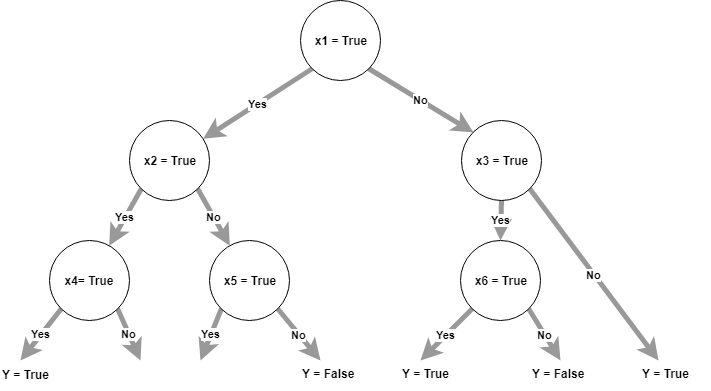
\includegraphics[width=0.75\textwidth]{design_and_methodology/decisiontree.png}}
\caption{\label{fig:decisiontree} An example of a Decision Tree Classifier.}
\end{figure}

The Decision Tree Classifier is a simple classification algorithm that can be used for binary or multi-class classification. DT classifiers learn simple decision rules based on the attributes of the training data. These decision rules form a tree structure (Figure ~\ref{fig:decisiontree}) which is used to predict the value of a target variable. The leaf nodes represent the class labels. When an unclassified document is received questions are asked until a leaf node is reached and the document is assigned that class.\newline\newline

The DT Classifier was implemented using Scikit Learn with the following parameters:

\begin{tcolorbox}
\begin{center}
	DecisionTreeClassifier (criterion='entropy', max\_depth=32, max\_features=None, min\_samples\_leaf=2, min\_samples\_split=0.1)
\end{center}
\end{tcolorbox}

\subsubsection*{Random Forest}

The Random Forest Classifier is an ensemble classification algorithm, meaning it combines multiple base classification algorithms. It consists of multiple DT classifiers. The final class prediction is calculated by getting the average of the decisions of the individual decision trees.

The RF Classifier was implemented using Scikit Learn with the following parameters:

\begin{tcolorbox}
\begin{center}
	RandomForestClassifier (n\_estimators=500, max\_features='log2', criterion='entropy')
\end{center}
\end{tcolorbox}

\subsubsection*{Multi Layer Perceptron}

The Multi Layer Perceptron Classifier is a deep, feedforward, artificial neural network. It consists of a minimum of three layers (Figure ~\ref{fig:mlp}): an input layer, a hidden layer and an output layer. The input layer receives the data, the output layer makes a decision and the hidden layers approximate the function.

The MLP classifier learns a function by based on the training set. Given a set of features $X = x_1,x_2,x_3,...,x_n$ and a target y, it learns a non-linear approximation function. Backpropagation is used to train the MLP Classifier.

\begin{figure}[h!]
\centering
\fbox{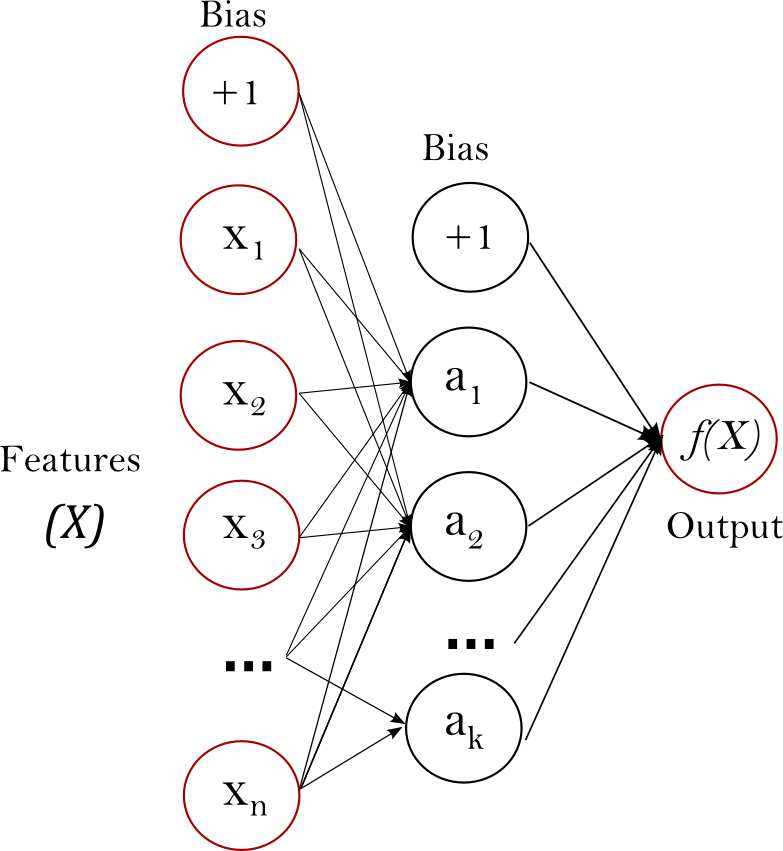
\includegraphics[width=0.5\textwidth]{design_and_methodology/multilayerperceptron_network.png}}
\caption{\label{fig:mlp} A Multi Layer Perceptron Classifier with one hidden layer \cite{scikit-learn}.}
\end{figure}

The MLP Classifier was implemented using Scikit Learn with the following parameters:

\begin{tcolorbox}
\begin{center}
	MLPClassifier (alpha=1,activation='identity', hidden\_layer\_sizes=(100,), learning\_rate='constant', solver='adam')
\end{center}
\end{tcolorbox}

\subsubsection*{Logistic Regression}

The Logistic Regression Classifier is a linear classification algorithm that uses the logistic function to model the training data. The logistic function is as follows:
\begin{equation}
  g(z)= \frac{1}{(1+e^{-z})}  
\end{equation}

The LR Classifier was implemented using Scikit Learn with the following parameters:

\begin{tcolorbox}
\begin{center}
	LogisticRegression (C=1,multi\_class='multinomial',penalty='l2',solver='saga')
\end{center}
\end{tcolorbox}

\subsubsection*{Support Vector Machine}

The Support Vector Machine Classifier is a discriminative classifier (Figure ~\ref{fig:svm}). It finds the optimum hyperplane that separates the data into the labelled classes. It aims to maximise the distance between the hyperplane and the support vectors (the points closest to the hyperplane).

\begin{figure}[h!]
\centering
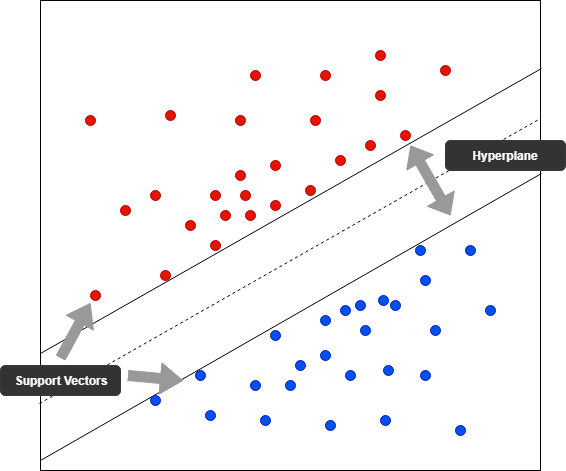
\includegraphics[width=0.75\textwidth]{design_and_methodology/svm.png}
\caption{\label{fig:svm} An example of a Support Vector Machine Classifier.}
\end{figure}

The SVM Classifier was implemented using Scikit Learn with the following parameters:

\begin{tcolorbox}
\begin{center}
	SVC (C=10.1,decision\_function\_shape='ovo',degree=1,gamma=1,kernel='rbf')
\end{center}
\end{tcolorbox}

\subsubsection*{K Nearest Neighbours}

\begin{figure}[h!]
\centering
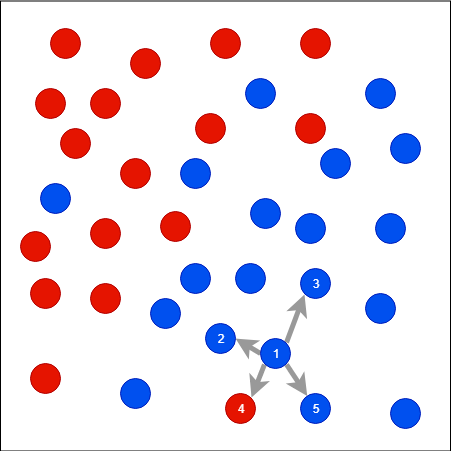
\includegraphics[width=0.7\textwidth]{design_and_methodology/knn.png}
\caption{\label{fig:knn} An example of a K Nearest Neighbours Classifier.}
\end{figure}

The K Nearest Neighbours Classifier doesn't build a model like other classification algorithms. It uses a majority vote of the "nearest neighbours" to a document. A label is assigned to a document based on the class that has the majority of the nearest neighbours to the document. For example in Figure ~\ref{fig:knn}, point one would be assigned the label blue. Taking it's four nearest neighbours it has three blue neighbours and one red neighbour. The point is assigned to the class with the majority of the nearest neighbour, blue.

The KNN Classifier was implemented using Scikit Learn with the following parameters:

\begin{tcolorbox}
\begin{center}
	KNeighborsClassifier(n\_neighbors=17,algorithm='ball\_tree',weights='distance',
	leaf\_size=10,p=2)
\end{center}
\end{tcolorbox}

\subsubsection*{Gaussian Process}

The Gaussian Process Classifier implements Gaussian Processes for classification. Gaussian Processes are probability distributions over possible functions.

The definition of a Gaussian Process is: $P(f)$ is a Gaussian process if for any finite subset $\{x_1,x_2,...,x_n\} \subset X$, the marginal distribution over that finite subset $P(f)$ has a multivariate Gaussian distribution.

The GP Classifier puts a Gaussian Process on a latent function, which is then squashed through a link function to get the probabilistic classification. For classification, the posterior of the latent function is not Gaussian, instead the logit function is used. A Gaussian likelihood function is inappropriate for discrete class labels \cite{gaussianProcesses2006}.

The GP Classifier was implemented using Scikit Learn with the following parameters:

\begin{tcolorbox}
\begin{center}
	GaussianProcessClassifier(kernel=1.0 * RBF(1.0), optimizer='fmin\_l\_bfgs\_b')
\end{center}
\end{tcolorbox}

\subsubsection*{Adaboost}

The AdaBoost Classifier is another ensemble classification algorithm, introduced by Freund and Schapire \cite{adaboost1997}.

The AB Classifier works by fitting a series of weak base classifiers on incrementally re-weighted versions of the training data. The predictions from the base classifiers are combined with a majority vote or sum, to get an overall classification. The 'boosting' component of the algorithm involves re-weighting the data on each iteration. Samples that were predicted correctly have their weight increased and samples that were predicted incorrectly have their weight decreased.

The AB Classifier was implemented using Scikit Learn with the following parameters:

\begin{tcolorbox}
\begin{center}
	AdaBoostClassifier(base\_estimator=None, n\_estimators=50,learning\_rate=1, algorithm=’SAMME.R’)
\end{center}
\end{tcolorbox}

Scikit Learn's version of AdaBoost implements the SAMME (Stagewise Additive Modeling using a Multi-class Exponential loss function) algorithm \cite{multiclassada2009}.

\subsubsection*{Gaussian Naive Bayes}

The Gaussian Naive Bayes Classifier is one of a set of Naive Bayes Classification algorithms. All of the Naive Bayes classifiers are based applying Bayes Rule along with the ‘naive’ assumption that features are conditionally independent. Bayes Rule: 
\begin{center}
\(P(A\mid B)=\frac{P(B\mid A)\:P(A)}{P(B)}\). 
\end{center}
In the GNB Classifier the likelihood of the features is assumed to be Gaussian:
\begin{center}
$P(x_i|y) = \frac{1}{\sqrt{2\pi\sigma_y^2}} exp (- \frac{(x_i - \mu_y)^2}{2\sigma_y^2})$
\end{center}
The GNB Classifier was implemented using Scikit Learn with the following parameters:

\begin{tcolorbox}
\begin{center}
	GaussianNB (priors=None, var\_smoothing=1e-09)
\end{center}
\end{tcolorbox}

\subsubsection*{Bernoulli Naive Bayes}

The Bernoulli Naive Bayes Classifier is another of the Naive Bayes Classification algorithms. The BNB Classifier implements the Naive Bayes algorithm for data that is distributed according to multivariate Bernoulli distributions. It has been seen to work better than the GNB Classifier on shorter texts.

The decision rule for the BNB Classifier is:
\begin{center}
$P(x_i|y) = P(i|y)x_i + (1 - P(i|y))(1 - x_i)$
\end{center}

The BNB Classifier was implemented using Scikit Learn with the following parameters:

\begin{tcolorbox}
\begin{center}
	BernoulliNB (alpha=1.0, binarize=0.0, class\_prior=None, fit\_prior=True)
\end{center}
\end{tcolorbox}

\subsubsection*{Multinomial Naive Bayes}

The Multinomial Naive Bayes Classifier is another of the Naive Bayes Classification algorithms. MNB implements the Naive Bayes algorithm for multinomial distributed data.

The MNB Classifier was implemented using Scikit Learn with the following parameters:

\begin{tcolorbox}
\begin{center}
	MultinomialNB(alpha=1.0, class\_prior=None, fit\_prior=True)
\end{center}
\end{tcolorbox}

\subsubsection*{Quadratic Discriminant Analysis and Linear Discriminant Analysis}

\begin{figure}[h!]
\centering
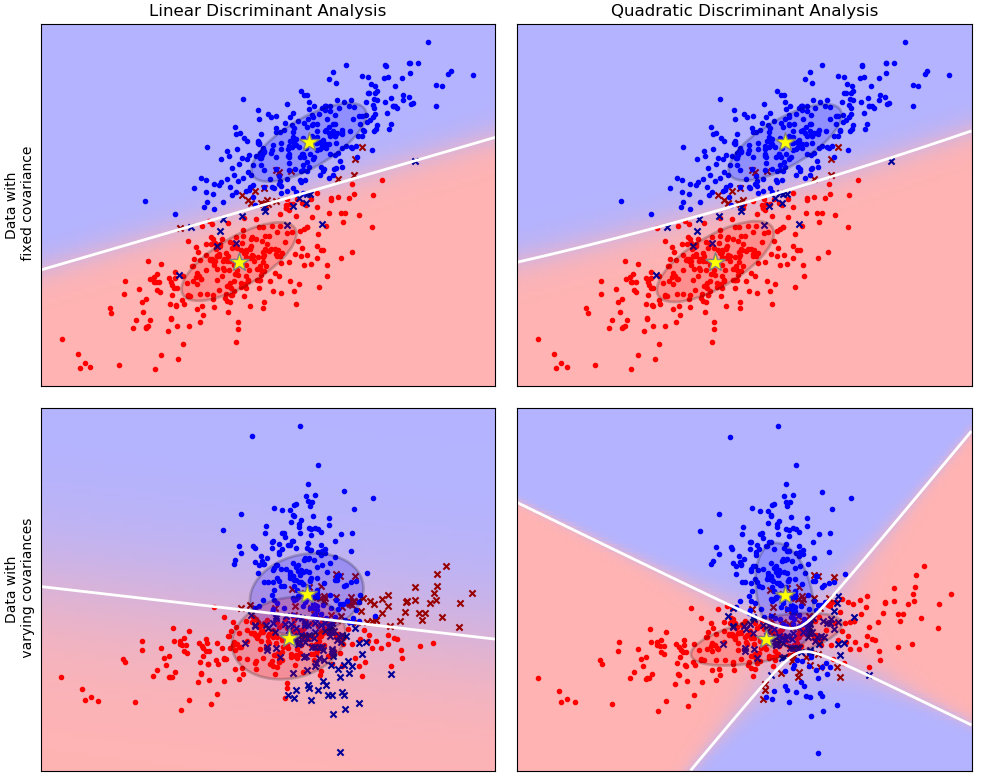
\includegraphics[width=0.9\textwidth]{design_and_methodology/qda_and_lda.png}
\caption{\label{fig:qdalda} Boundaries of the Quadratic Discriminant Analysis and Linear Discriminant Analysis Classifiers \cite{scikit-learn}.}
\end{figure}

The Quadratic Discriminant Analysis Classifier and the Linear Discriminant Analysis Classifier, have a quadratic and linear decision surface, respectively. QDA is more flexible as it can learn quadratic boundaries, LDA can only learn linear boundaries (Figure ~\ref{fig:qdalda}). 

Both the QDA and the LDA Classifier were implemented using Scikit Learn with the folllowing parameters:

\begin{tcolorbox}
\begin{center}
	QuadraticDiscriminantAnalysis(priors=None, reg\_param=0.0, store\_covariance=False, store\_covariances=None, tol=0.0001)
\end{center}
\end{tcolorbox}

\begin{tcolorbox}
\begin{center}
	LinearDiscriminantAnalysis(n\_components=None, priors=None, shrinkage=None, solver='svd', store\_covariance=False, tol=0.0001)
\end{center}
\end{tcolorbox}


\section{Sentiment Analysis}

Once the tweets had been classified as reviews, sentiment analysis was performed on them. Sentiment analysis is the process of identifying the opinion expressed about a particular subject in some text. The goal is to determine whether the opinion is positive, negative or neutral, and to what extent. 

The Stanford NLP Sentiment Analyser \cite{stanfordSentiment2013} was used to classify the sentiment of the tweets. The Stanford NLP Sentiment Analyser was chosen as it is the dominant NLP library used in research in this area. It has achieved 85.4\% accuracy in single sentence positive/negative classification. 

\subsection{The Stanford NLP Sentiment Analyser}

The Stanford Sentiment Analyser is based on a Recursive Neural Tensor Network. It was trained on a sentiment treebank of movie reviews from the movie review site RottenTomatoes. The treebank consists of sentences which are annotated on a phrase level. 

The Stanford NLP Sentiment Analyser has it's limitations. Due to the fact that it was trained on movie reviews and is being applied to tweets, optimum performance is not achieved. The best performance would be achieved if the Sentiment Analyser was re-trained on a dataset as similar to ours as possible. Ideally the Sentiment Analyser would be re-trained with a set of hotel related tweets. This would involve manually annotating a collection of tweets at a phrase level to produce a treebank. This is an area for future research.

The Stanford NLP Sentiment Analyser classifies the text into one of the following five sentiment judgements: 
\begin{enumerate}
    \item Very Negative
    \item Negative
    \item Neutral
    \item Positive
    \item Very Positive
\end{enumerate}

The output from the Sentiment Analyser for a tweet looks like this:

\begin{lstlisting}[
caption={Output from Stanford NLP Sentiment Analyser},
captionpos=b,label=lst:stanfordoutput,language=json,firstnumber=1]
"sentimentValue": "3",
"sentiment": "Positive",
"sentimentDistribution": [
    0.03910365552553,
    0.18375415309071,
    0.26346977003905,
    0.42548434014862,
    0.0881880811961
]
\end{lstlisting}

The sentiment value (3) and sentiment (Positive) define the class the tweet has been assigned (Listing ~\ref{lst:stanfordoutput}). In this case the tweet is positive. The sentiment distribution shows how strongly the tweet aligns with each class, from very negative to very positive. This tweet has a maximum value of 0.42548434014862 so it is assigned the positive label.

\subsection{Normalisation}

The sentiment scores produced by the Stanford NLP Sentiment Analyser were produced per tweet. They needed to be normalised so that they were per hotel and lay between zero and one.

A majority voting technique was used to normalise the scores. For each hotel we had a selection of tweets. These tweets are divided into five clusters; very negative, negative, neutral (ignored), positive and very positive. A mean value was calculated for each cluster. This was calculated by summing the corresponding score in the sentiment distribution for each tweet and dividing by the number of tweets in the cluster. The class with the highest mean value was assigned to the hotel.

There were some cases where tweets related to a hotel chain, for example Hilton Hotels, rather than an individual Hilton Hotel, for example Hilton Dublin Kilmainham. In these cases sentiment scores were generated for the chain as a whole. The score for the chain was assigned to each hotel in the chain. This only happened in the cases where we had no information about the individual hotel but had information about the chain as a whole, in an attempt to boost the numbers of hotels we had sentiment scores for. The problem is that one Hilton Hotel could be amazing and another could be terrible. Ideally more data would be collected so that every hotel had it's own individual sentiment score.

This mean score was then normalised between zero and one, with the following weighting.
\begin{itemize}
    \item Very Negative: 0 --> 0.25
    \item Negative: 0.25 --> 0.5
    \item Positive: 0.5 --> 0.75
    \item Very Positive: 0.75 --> 1
\end{itemize}

The following max-min normalisation formulae were used:

\begin{tcolorbox}[title=Normalisation]
$Normalised\ Score\ (-) = max\ score-(actual\ score \times (max\ score - min\ score))$
$Normalised\ Score\ (+) = (actual\ score \times (max\ score - min\ score)) + min\ score$
\end{tcolorbox}

Taking the tweet above with a positive score of 0.42548434014862 as an example:
\begin{tcolorbox}[title=Example]
$Normalised\ score\ (Positive) = (0.42548434014862\ \times\ (0.75\ -\ 0.5)) + 0.5.$
$Normalised\ score\ (Positive) = 0.606$
\end{tcolorbox}

\section{CoRE Recommender System}

The sentiment scores produced by the Stanford NLP Sentiment Analyser \cite{stanfordSentiment2013} were used to re-rank the list of hotel recommendations produced by the CoRE Recommender System \cite{core2019}. CoRE is a Cold Start Resistant and Extensible Recommender system, developed in collaboration with Ryanair. 

\subsection{CoRE}

The CoRE recommender is an algorithmic approach to hotel recommendation. It can function in extreme cold start conditions. CoRE is a hybrid recommender that makes use of collaborative filtering, content-based recommendation and contextual suggestion. It is made up of three models, a user model, a segment model and a context model. Each model is generated as a weighted feature vector.

The user model takes hotel features from Expedia, such as Free Wi-Fi, Free Breakfast, Restaurant, Hair dryer, etc. and uses them to build a vector of features describing a hotel. A vector of features is stored for each hotel. Then, for each user who has a previous hotel booking, the user model is constructed by weighting the features of the hotels that the user has booked before.

The segment model introduces collaborative filtering to the recommender. Collaborative filtering methods recommend to users based on the preferences of similar users. The segment model is constructed as a weighted vector of features of hotels that have been booked by all users from a specific segment. A segment is a group of similar users. Users are assigned to a segment based on their flight booking history.

The context model uses contextual information to recommend hotels to the user. The contextual information used is the trip type specified by the user on their flight booking. If trip type information is not available it can be inferred by the number of people travelling with the user, for example, two adults and two children indicates a family trip. The context model is constructed as a weighted vector of features of hotels that have been booked by all users who had the same trip type.

\begin{figure}[h!]
\centering
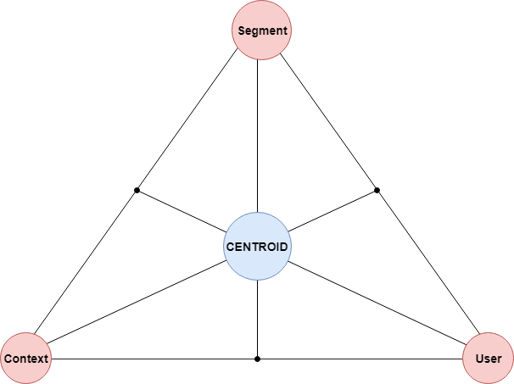
\includegraphics[width=0.5\textwidth]{design_and_methodology/centroid.png}
\caption{\label{fig:centroid} Centroid of CoRE Models.}
\end{figure}

The three models are combined by calculating the centroid vector (Figure ~\ref{fig:centroid}). A weighting is applied to determine the effect of each model in the final vector. The cosine similarity between the vector of each hotel and the centroid vector of the user is then calculated, and a list of hotels is produced. The hotels are ranked based on the similarity score. CoRE is easily extensible. A fourth model could easily be added and incorporated into the centroid calculation.

CoRE was evaluated against the ranking approach currently used by Ryanair. Hotels from the target city are sorted based on their sequence number which is given to them by Expedia. The sequence number is based on the transactional data from the last 30 days. CoRE significantly outperforms this baseline, which is labelled 'Sequence' in Figure ~\ref{fig:coreperform}. CoRE achieves a mean percentile rank (MPR) of 22.04\% without feature weighting and 18.27\% with feature weighting.

\begin{figure}[h!]
\centering
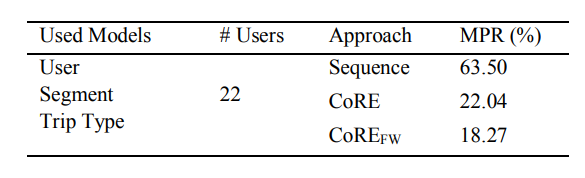
\includegraphics[width=0.75\textwidth]{design_and_methodology/core_results.PNG}
\caption{\label{fig:coreperform} Performance of CoRE with multiple models.}
\end{figure}

\subsection{Re-Ranking}

The scores produced by the Stanford NLP Sentiment Analyser were used to re-rank the list of hotels produced by the CoRE. This was done by simply multiplying the score of the hotel in the CoRE ranked list by the normalised sentiment score. The sentiment score normalised between zero and one boosts the score of hotels with a positive sentiment score and drags down the score of the hotels with a negative sentiment score.

\begin{equation}
    SentiCoRE\ Score = Sentiment\ Score \times CoRE\ Score
\end{equation}